\chapter{Introduction}\label{sec:introduction}

\section{Quantum Bits}
\label{subsec:qubits}

INTRODUCE CONCEPT OF DROPPING GLOBAL PHASE SOMEWHERE!

\subsection{Single Qubit Systems}
\label{subsubsec:qubits}
%Classical computers manipulate bits and the quantum equivalent is called a quantum bit, often abbreviated as qubit.
Classical computers manipulate bits, whereas quantum computer's most fundamental unit is called a quantum bit, often abbreviated as qubit. Bits as well as qubits are binary entities, meaning they can only take the values 0 and 1. A classical non-probabilistic bit can only be in one of the two possible states at once. In contrast, qubits obey the laws of quantum mechanics, which gives rise to the powerful property that - besides being a definite 0 or 1 - they can also be in a superposition of the two states. Mathematically this is expressed as a linear combination of the states 0 and 1:
\begin{equation}
\label{equ: simplequbit}
\ket{\psi} = \alpha \ket{0} + \beta \ket{1}
\end{equation}
where $\alpha$ and $\beta$ are complex coefficients ($\alpha, \beta \in \mathbb{C}$) and are often referred to as phase factors or amplitudes. \0 is the Dirac notation for the qubit being in state 0 and it represents a two-dimensional vector in a complex 2-D vector space (called Hilbert space $\mathcal{H}_{2}$). \0 and \1 are the computational basis states and they constitute an orthonormal basis of $\mathcal{H}_{2}$. For the sake of clarity, \0 and \1 can be thought of as the 2-D vectors shown below.
\begin{equation}
\label{equ: 0and1kets}
\ket{0} =  \colvec{1\\0} \quad \quad \ket{1} = \colvec{0\\1}
\end{equation}

Subbing these vectors into Equ.~\ref{equ: simplequbit} yields the vector representation of $\ket{\psi}$:
\begin{equation}
\label{equ: simplequbitvector}
\ket{\psi} = \alpha \colvec{1\\0} + \beta \colvec{0\\1} = \colvec{\alpha\\\beta}
\end{equation}

However, even though a qubit can be in a superposition of \0 and \1, when measured it will take the value \0 with a probability of
\begin{equation}
\label{equ:bornrule0}
Prob(\ket{0}) = {|\alpha|}^{2}
\end{equation}
and \1 with a probability of 
\begin{equation}
\label{equ:bornrule1}
Prob(\ket{1}) = {|\beta|}^{2}
\end{equation}

The fact that the probability of measuring a particular state is equal the absolute value squared of the respective amplitude is called Born's rule (citation). Since the total probability of measuring any value has to be 1, the following normalization condition must be satisfied:
\begin{equation}
\label{equ: normalization}
{|\alpha|}^{2} + {|\beta|}^{2} =  1
\end{equation}
Therefore, a qubit is inherently probabilistic but when measured it collapses into a single classical bit (0 or 1). It follows that a measurement destroys information about the superposition of the qubit (the values of $\alpha$ and $\beta$). This constitutes one of the main difficulties when designing quantum algorithms since only limited information can be obtained about the final states of the qubits in the quantum computer.

Using spherical polar coordinates, a single qubit can be visualized on the so-called Bloch sphere by parameterising $\alpha$ and $\beta$ in Equ.~\ref{equ: simplequbit} as follows:

\begin{equation}
\label{equ: blochqubit}
\ket{q} = \cos\frac{\theta}{2} \ket{0} + e^{i \phi} \sin\frac{\theta}{2} \ket{1}
\end{equation}

The Bloch sphere has a radius of 1 and is therefore a unit sphere. The \0 qubit state is defined to lie along the positive z-axis ($\hat{z}$) and the \1 state is defined to lie along the negative z-axis ($-\hat{z}$) as labelled in Fig.~\ref{fig:blochsphere}. At this point, it is important to note that these two states are mutually orthogonal in $\mathcal{H}_{2}$ even though they are not orthogonal on the Bloch sphere. 

Qubit states on the Bloch equator such as the $\hat{x}$ and $\hat{y}$ coordinate axes represent equal superpositions where \0 and \1 both have measurement probabilities equal to $0.5$. The $\hat{x}$-axis for example represents the equal superposition $\ket{q} = \frac{1}{\sqrt{2}} \ket{0} + \frac{1}{\sqrt{2}} \ket{1}$. As illustrated in Fig.~\ref{fig:blochsphere} any arbitrary 2-D qubit state $\ket{\psi}$ can be decomposed into the polar angles $\theta$ and $\phi$ and visualized as a vector on the Bloch sphere. Such an object is called the Bloch vector of the qubit state $\ket{\psi}$. The Bloch sphere will be the main visualization tool for qubit manipulations in this thesis.

\begin{figure}[!ht]
       \centering
       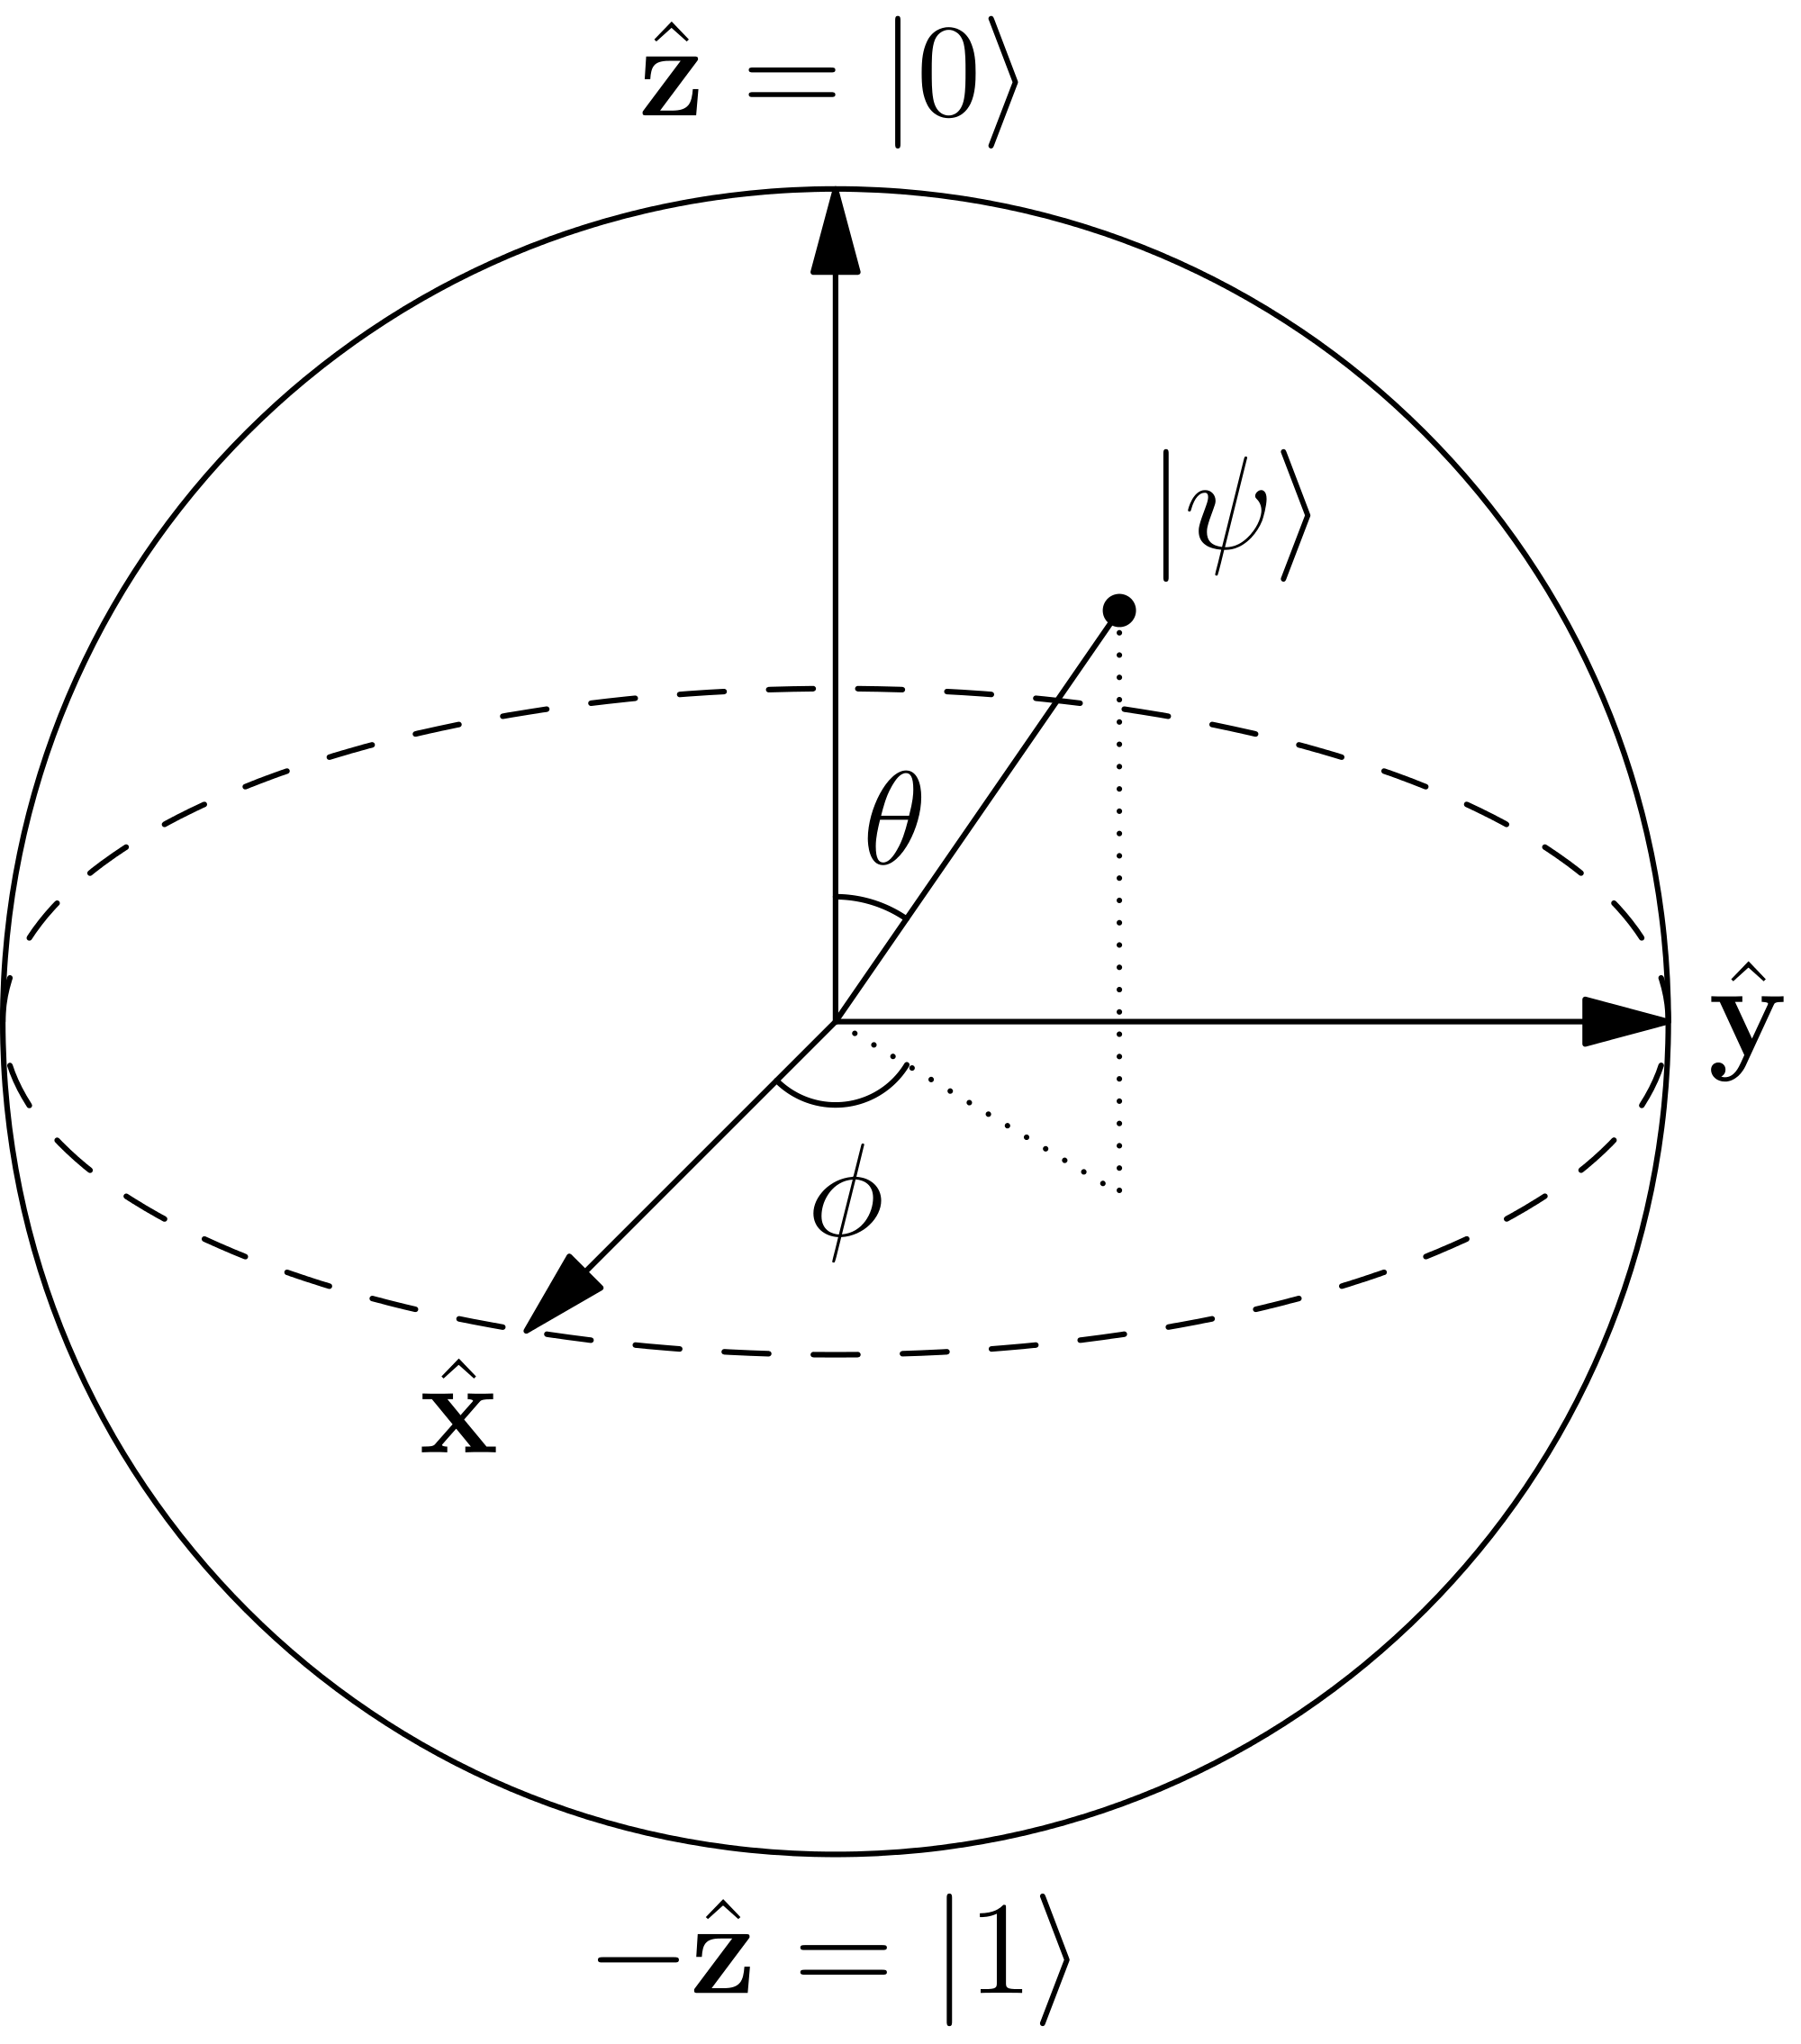
\includegraphics[scale=0.07]{img/blochsphere.png}
       \caption{\label{fig:blochsphere} An arbitrary two-dimensional qubit $\ket{\psi}$ visualized on the Bloch sphere.$^{1}$}
\end{figure}

\footnotetext[1]{Reprinted from Wikipedia, n.d., Retrieved September 7, 2016, from \url{https://en.wikipedia.org/wiki/Bloch_Sphere}. Copyright 2012 by Glosser.ca. Reprinted with permission.}

\subsection{Multiple Qubit Systems}
\label{subsec:multiplequbitsystems}

Introduce tensor products here!

\subsection{Entanglement}
\label{subsec:entanglement}

Introduce entanglement and non-factorising tensor states here!

%%%%% SECTION: Q LOGIC GATES


\section{Quantum Logic Gates}
\label{subsec:quantumlogicgates}
In order to perform quantum computations, tools, analogous to the classical logic gates, are needed for qubit manipulation. Quantum logic gates are square matrices that can be visualized as rotations on the Bloch sphere. The following subsections will introduce the major single and multi qubit logic gates.

\subsection{Single Qubit Gates}
\label{subsubsec:singlequbitgates}

ADD THE CIRCUIT REPRESENTATIONS OF THE RESPECTIVE GATES!

In the following section we will evaluate the action of the most common single qubit gates on an arbitrary qubit state $\ket{\psi}$ defined in Equ.~\ref{equ: simplequbitvector}.

%The four most basic single-qubit quantum gates are given by the four Pauli matrices listed below in Equ. ~\ref{equ: paulimatrices}.

%\begin{align}
%\label{equ: paulimatrices}
%\sigma_{0} &= \mathbb{1} = \begin{pmatrix}
% 1 & 0 \\ 
% 0 & 1
% \end{pmatrix}
% \quad
% &&\sigma_{1} = \sigma_{x} = \begin{pmatrix}
% 0 & 1 \\ 
% 1 & 0
% \end{pmatrix}
% \nonumber
% \\
% \sigma_{2} &= \sigma_{y} = \begin{pmatrix}
% 0 & -i \\ 
% i & 0
% \end{pmatrix}
% \quad
% &&\sigma_{3} = \sigma_{z} = \begin{pmatrix}
% 1 & 0 \\ 
% 0 & -1
% \end{pmatrix}
%\end{align}

\subsubsection{Identity Gate}
\label{subsubsubsec:identitygate}

The simplest quantum gate is the identity or idle gate given by the 0\textsuperscript{th} Pauli matrix:

\begin{equation}
\sigma_{0} = \mathbb{1} = \begin{pmatrix}
 1 & 0 \\ 
 0 & 1
 \end{pmatrix}
\end{equation}

The action of a quantum gate on a qubit state can be analysed using the gate's matrix and the qubit's vector representation. Applying some straightforward linear algebra in this case yields:

\begin{equation}
\label{equ:identityverification}
\mathbb{1} \otimes \ket{\psi} = \mathbb{1} \otimes (\alpha \ket{0} + \beta \ket{1}) = \begin{pmatrix}
 1 & 0 \\ 
 0 & 1
 \end{pmatrix} \begin{pmatrix}
 \alpha  \\ 
 \beta
 \end{pmatrix} = \begin{pmatrix}
 \alpha  \\ 
 \beta
 \end{pmatrix} = \alpha \ket{0} + \beta \ket{1} = \ket{\psi}
\end{equation}

Hence, applying the identity gate to an arbitrary qubit state $\ket{\psi}$ leaves the state unchanged as shown in Equ.~\ref{equ:identityverification}. The idle gate is mainly used for measuring the error and lifetimes of qubits since it only evolves the qubit in time without actively rotating its Bloch vector.

\subsubsection{Qubit Flip (X) Gate}
\label{subsubsubsec:xgate}

The quantum equivalent of the classical NOT gate is called X gate and is given by the 1\textsuperscript{st} Pauli matrix:

\begin{equation}
\sigma_{1} = X = \begin{pmatrix}
 0 & 1 \\ 
 1 & 0
 \end{pmatrix}
\end{equation}

The action of the X gate is easily verified by performing some linear algebra,

\begin{equation}
\label{equ:xverification1}
X \otimes \ket{\psi} = X \otimes (\alpha \ket{0} + \beta \ket{1}) = \begin{pmatrix}
 0 & 1 \\ 
 1 & 0
 \end{pmatrix} \begin{pmatrix}
 \alpha  \\ 
 \beta
 \end{pmatrix} = \begin{pmatrix}
 \beta  \\ 
 \alpha
 \end{pmatrix} = \beta \ket{0} + \alpha \ket{1}
\end{equation}

Thus, applying the X gate to qubit state $\ket{\psi}$ swaps the amplitudes of \0 and \1. More specifically, applying X to the \0 state results in the \1 state,

\begin{equation}
\label{equ:xverification2}
X \otimes \ket{0} = \begin{pmatrix}
 0 & 1 \\ 
 1 & 0
 \end{pmatrix} \begin{pmatrix}
 1  \\ 
 0
 \end{pmatrix} = \begin{pmatrix}
 0  \\ 
 1 \end{pmatrix} =  \ket{1}
\end{equation}

And the \0 state is recovered when applying X again to the \1 state,

\begin{equation}
\label{equ:xverification3}
X \otimes \ket{1} = \begin{pmatrix}
 0 & 1 \\ 
 1 & 0
 \end{pmatrix} \begin{pmatrix}
 0  \\ 
 1
 \end{pmatrix} = \begin{pmatrix}
 1  \\ 
 0 \end{pmatrix} =  \ket{0}
\end{equation}

On the Bloch sphere, the X gate corresponds to a anti-clockwise $\pi$ rotation around the x-axis as shown in Fig.~\ref{img:blochxgate}.

\begin{figure}[ht]
   \centering
   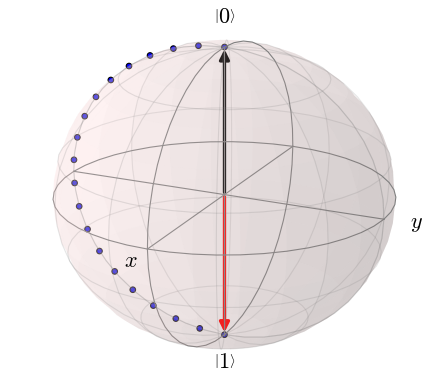
\includegraphics[width=0.5\textwidth]{img/blochxgate.png}
   \caption{Visualization of the X gate on the Bloch sphere. Initial state (black) transformed to final state (red).}
   \label{img:blochxgate}
\end{figure}

From Equ.~\ref{equ:xverification1},~\ref{equ:xverification2} and~\ref{equ:xverification3} it follows that X is its own inverse as well as its own Hermitian conjugate:
\begin{align}
XX &= XX^\dagger = \mathbb{1} \\
X &= X^{-1} = X^\dagger
\end{align}

\subsubsection{Phase Flip (Z) Gate}
\label{subsubsubsec:zgate}

The phase flip gate, often called Z gate, is a quantum logic gate without classical equivalent. Its matrix representation is given by the 3\textsuperscript{rd} Pauli matrix:

\begin{equation}
\sigma_{3} = Z = \begin{pmatrix}
 1 & 0 \\ 
 0 & -1
 \end{pmatrix}
\end{equation}

It acts on $\ket{\psi}$ as follows:

\begin{equation}
\label{equ:zverification1}
Z \otimes \ket{\psi} = Z \otimes (\alpha \ket{0} + \beta \ket{1}) = \begin{pmatrix}
 1 & 0 \\ 
 0 & -1
 \end{pmatrix} \begin{pmatrix}
 \alpha  \\ 
 \beta
 \end{pmatrix} = \begin{pmatrix}
 \alpha  \\ 
 -\beta
 \end{pmatrix} = \alpha \ket{0} - \beta \ket{1}
\end{equation}

Applying Z again recovers the initial state,

\begin{equation}
\label{equ:zverification2}
Z \otimes (\alpha \ket{0} - \beta \ket{1}) = \alpha \ket{0} + \beta \ket{1} = \ket{\psi}
\end{equation}

Fig.~\ref{img:blochzgate} visualizes that the Z gate corresponds to a anti-clockwise $\pi$ rotation around the z-axis.

\begin{figure}[ht]
   \centering
   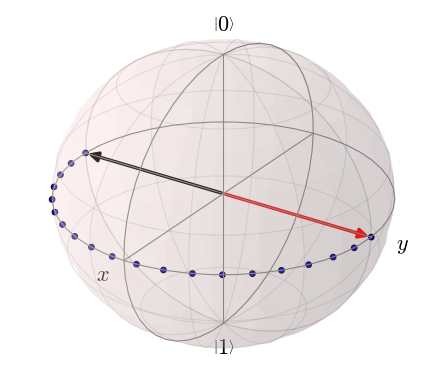
\includegraphics[width=0.5\textwidth]{img/blochzgate.png}
   \caption{Visualization of the Z gate on the Bloch sphere. Initial state (black) transformed to final state (red).}
   \label{img:blochzgate}
\end{figure}

From Equ.~\ref{equ:zverification1} and Equ.~\ref{equ:zverification2}, it follows that also Z is its own inverse as well as Hermitian conjugate:
\begin{align}
ZZ &= ZZ^\dagger = \mathbb{1} \\
Z &= Z^{-1} = Z^\dagger
\end{align}

\subsubsection{Qubit and Phase Flip (Y) Gate}
\label{subsubsubsec:ygate}

The combined qubit and phase flip gate, also called Y gate, is a quantum logic gate without classical equivalent since it involves the complex number i ($\sqrt{-1}$). Its matrix representation is given by the 2\textsuperscript{nd} Pauli matrix:

\begin{equation}
\sigma_{2} = Y = \begin{pmatrix}
 0 & -i \\ 
 i & 0
 \end{pmatrix}
\end{equation}

It essentially combines the action of the X and the Z gate since it exchanges the amplitudes and adds a phase to the qubit state:

\begin{equation}
\label{equ:yverification1}
Y \otimes \ket{\psi} = Y \otimes (\alpha \ket{0} + \beta \ket{1}) = \begin{pmatrix}
 0 & -i \\ 
 i & 0
 \end{pmatrix} \begin{pmatrix}
 \alpha  \\ 
 \beta
 \end{pmatrix} = \begin{pmatrix}
 -i\beta  \\ 
 i\alpha
 \end{pmatrix} = -i\beta \ket{0} + i\alpha \ket{1}
\end{equation}

One can simplify the last expression since a so-called global phase of $i$ is present which can be factored out:

\begin{equation}
\label{equ:yverification2}
-i\beta \ket{0} + i\alpha \ket{1} = i(-\beta \ket{0} + \alpha \ket{1}) = -\beta \ket{0} + \alpha \ket{1}
\end{equation}

To proof this, one calculates the probability of measuring the \0 state including the global phase (last expression in Equ.~\ref{equ:yverification1}) by taking the absolute value squared of the amplitude of the \0 state:

\begin{equation}
\label{equ:globalphase}
Prob(\ket{0}) = \mid-i\beta\mid^2 = (-i\beta)(i\beta) = -i^2\beta^2 = -(\sqrt{-1})^2\beta^2 = \beta^2
\end{equation}

When calculating the probability whilst omitting the global phase of $i$ one arrives at the same result: 

\begin{equation}
\label{equ:globalphase}
Prob(\ket{0}) = \mid-\beta\mid^2 = \beta^2
\end{equation}

It follows that a global phase is immeasurable in experiments and can therefore be left out.

The Y gate corresponds to a $\pi$ rotation around the y-axis of the Bloch sphere as shown in Fig.~\ref{img:blochygate}.

\begin{figure}[ht]
   \centering
   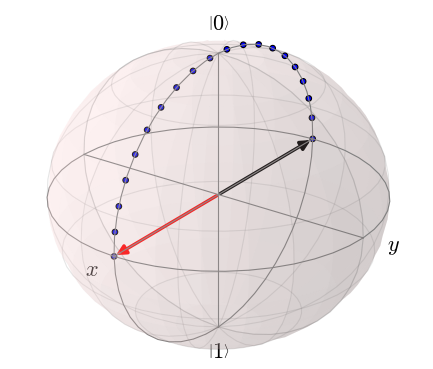
\includegraphics[width=0.5\textwidth]{img/blochygate.png}
   \caption{Visualization of the Y gate on the Bloch sphere. Initial state (black) transformed to final state (red).}
   \label{img:blochygate}
\end{figure}

From Equ.~\ref{equ:yverification1} it follows that, similar to the X and Z gate, the Y gate is its own inverse and Hermitian conjugate:

\begin{align}
YY &= YY^\dagger = \mathbb{1} \\
Y &= Y^{-1} = Y^\dagger
\end{align}


\subsubsection{Hadamard (H) Gate}
\label{subsubsubsec:hadamardgate}

In order to create superpositions from an initial \0 or \1 state the Hadamard or H gate is required. It is defined by the following matrix:

\begin{equation}
H = \begin{pmatrix}
 \frac{1}{\sqrt{2}} & \frac{1}{\sqrt{2}} \\ 
 \frac{1}{\sqrt{2}} & -\frac{1}{\sqrt{2}}
 \end{pmatrix}
\end{equation}

The action of the H gate is best understood when applying it to the \0 state,

\begin{equation}
\label{equ:hadamardverification1}
H \otimes \ket{0} = \begin{pmatrix}
 \frac{1}{\sqrt{2}} & \frac{1}{\sqrt{2}} \\ 
 \frac{1}{\sqrt{2}} & -\frac{1}{\sqrt{2}}
 \end{pmatrix} \begin{pmatrix}
 1 \\ 
 0
 \end{pmatrix} = \begin{pmatrix}
 \frac{1}{\sqrt{2}} \\ 
 \frac{1}{\sqrt{2}}
 \end{pmatrix} = \frac{1}{\sqrt{2}} \ket{0} + \frac{1}{\sqrt{2}} \ket{1}
\end{equation}

Thus, the H gate has transformed the \0 state into an equal superposition of \0 and \1. Similarly applying the H gate to the \1 state creates an equal superposition of \0 and \1 with an additional negative sign on the \1 state:

\begin{equation}
\label{equ:hadamardverification2}
H \otimes \ket{1} = \begin{pmatrix}
 \frac{1}{\sqrt{2}} & \frac{1}{\sqrt{2}} \\ 
 \frac{1}{\sqrt{2}} & -\frac{1}{\sqrt{2}}
 \end{pmatrix} \begin{pmatrix}
 0 \\ 
 1
 \end{pmatrix} = \begin{pmatrix}
 \frac{1}{\sqrt{2}} \\ 
 -\frac{1}{\sqrt{2}}
 \end{pmatrix} = \frac{1}{\sqrt{2}} \ket{0} - \frac{1}{\sqrt{2}} \ket{1}
\end{equation}

Fig.~\ref{img:blochhgate} illustrates how the H gate first rotates the qubit around the y-axis by $\frac{\pi}{2}$ radians followed by a $\pi$ rotation around the x-axis.

\begin{figure}[ht]
   \centering
   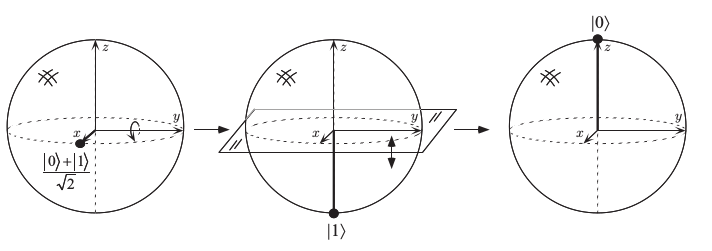
\includegraphics[width=0.8\textwidth]{img/blochhadamardnielsenchuang.png}
   \caption{Visualization of the Hadamard gate on the Bloch sphere, acting on the input state $\ket{q} = \frac{1}{\sqrt{2}} \ket{0} + \frac{1}{\sqrt{2}} \ket{1}$.\textsuperscript{2}}
   \label{img:blochhgate}
\end{figure}

\footnotetext[2]{Reprinted from Michael A. Nielsen and Isaac L. Chuang. Quantum Computation and Quantum Information. Cambridge University Press, 2000. Copyright 2010 by Nielsen \& Chuang.}

%\begin{figure}[ht]
%   \centering
%   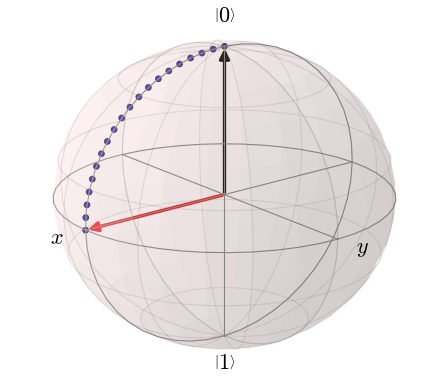
\includegraphics[width=0.5\textwidth]{img/blochhadamard.png}
%   \caption{Visualization of the H gate on the Bloch sphere. Initial state (black) transformed to final state (red).}
%   \label{img:blochhgate}
%\end{figure}

Omitting the proof, from Equ.~\ref{equ:hadamardverification1} and Equ.~\ref{equ:hadamardverification2} one can easily see that the H gate is a Hermitian matrix which means it is its own Hermitian conjugate and inverse:

\begin{align}
HH &= HH^\dagger = \mathbb{1} \\
H &= H^{-1} = H^\dagger
\end{align}

\subsubsection{$\frac{\pi}{2}$ Rotation (S,S$^\dagger$) Gates}
\label{subsubsubsec:cliffordgates}

The S and S$^\dagger$ gates make it possible to reach more points on the Bloch sphere since they introduce $\frac{\pi}{2}$ rotations around the z-axis. The S gate is defined to be the square root of the Z gate and it is not Hermitian giving rise to the following two matrices: 

\begin{equation}
S = \sqrt{Z} = \begin{pmatrix}
 1 & 0 \\ 
 0 & i
 \end{pmatrix}
 \quad \quad \quad \quad
S^\dagger = \begin{pmatrix}
 1 & 0 \\ 
 0 & -i
 \end{pmatrix}
\end{equation}

The S gate simply adds an imaginary phase to the \1 state,

\begin{equation}
\label{equ:sverification}
S \otimes \ket{\psi} = S \otimes (\alpha \ket{0} + \beta \ket{1}) = \begin{pmatrix}
 1 & 0 \\ 
 0 & i
 \end{pmatrix} \begin{pmatrix}
 \alpha  \\ 
 \beta
 \end{pmatrix} = \begin{pmatrix}
 \alpha  \\ 
 i\beta
 \end{pmatrix} = \alpha \ket{0} + i\beta \ket{1}
\end{equation}

Visually this corresponds to a $\frac{\pi}{2}$ rotation around the z-axis as shown in Fig.~\ref{img:blochsgate}. In contrast, the S$^\dagger$ gate performs the inverse action and therefore rotates the qubit by $-\frac{\pi}{2}$ radians around the z-axis.

\begin{figure}[ht]
   \centering
   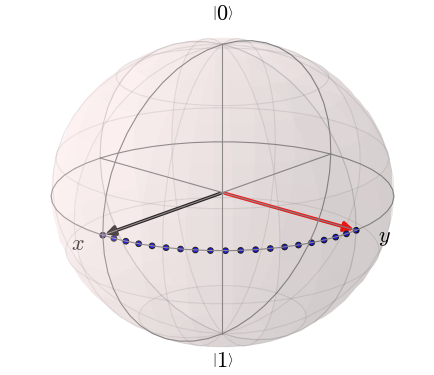
\includegraphics[width=0.5\textwidth]{img/blochsgate.png}
   \caption{Visualization of the S gate on the Bloch sphere. Initial state (black) transformed to final state (red).}
   \label{img:blochsgate}
\end{figure}

In contrast to all previously introduced gates, the S gate is not its own inverse or Hermitian conjugate. However, applying the S gate four times yields the identity matrix since it corresponds to a $2\pi$ rotation around the z-axis,

\begin{equation}
SSSS = \mathbb{1} = SS^\dagger
\end{equation}

\subsubsection{$\frac{\pi}{4}$ Rotation (T,T$^\dagger$) Gates}
\label{subsubsubsec:noncliffordgates}

Until this point, all introduced single qubit gates are part of the so-called Clifford group. The Gottesmann-Knill theorem states that all quantum circuits consisting only of Clifford gates can be efficiently simulated on a classical computer (citation!). To harness the full potential of quantum computation, one needs to add a non-Clifford gate to the quantum gate set. The T and T$^\dagger$ gates are such non-Clifford gates and are defined as follows,

\begin{equation}
T = \sqrt{S} = \begin{pmatrix}
 1 & 0 \\ 
 0 & e^{\frac{i\pi}{4}}
 \end{pmatrix}
\quad \quad \quad \quad
T^\dagger = \begin{pmatrix}
 1 & 0 \\ 
 0 & e^{-\frac{i\pi}{4}}
 \end{pmatrix}
\end{equation}

On the Bloch sphere, the T gate corresponds to a $\frac{\pi}{4}$ rotation around the z-axis as it can be seen in Fig.~\ref{img:blochtgate}. Consequently, the T$^\dagger$ gate constitutes a $-\frac{\pi}{4}$ rotation around the z-axis.

\begin{figure}[ht]
   \centering
   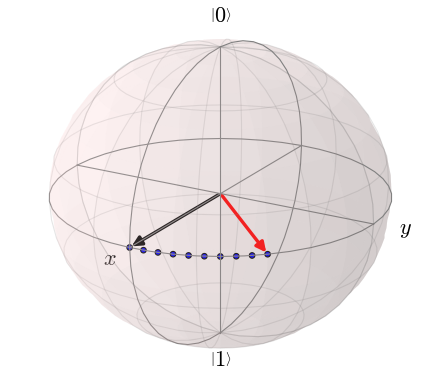
\includegraphics[width=0.5\textwidth]{img/blochtgate.png}
   \caption{Visualization of the T gate on the Bloch sphere. Initial state (black) transformed to final state (red).}
   \label{img:blochtgate}
\end{figure}

Similar to the S gate, applying the T gate eight times yields the identity matrix since eight $\frac{\pi}{4}$ rotations make a full $2\pi$ z-rotation.

\begin{equation}
TTTTTTTT = \mathbb{1} = TT^\dagger
\end{equation}

%%%%% SUBSECTION: MULTIPLE Q LOGIC GATES


\subsection{Multiple Qubit Gates}
\label{subsubsec:multiqubitgates}

\subsubsection{Controlled NOT Gate}
\label{subsubsubsec:cnotgate}

The most important two-qubit quantum gate is the controlled NOT or CNOT gate given by the following 4x4 matrix:
\begin{equation}
CNOT = \begin{pmatrix}
 \mathbb{1} & 0 \\ 
 0 & X
 \end{pmatrix} = \begin{pmatrix}
 1 & 0 & 0 & 0 \\ 
 0 & 1 & 0 & 0 \\
 0 & 0 & 0 & 1 \\
 0 & 0 & 1 & 0 \\
 \end{pmatrix}
\end{equation}

The CNOT gate takes two qubits, control and target qubit, as input. If and only if the control qubit is in the \1 state, the NOT (X) gate is applied to the target qubit. In equations, the CNOT will always be followed by parantheses containing the control qubit followed by the target qubit (e.g. CNOT(0,1)). The input-output relation for the CNOT gate is given in Table~\ref{tab:cnottruthtable} below.

\begin{table}[ht!]
\begin{center}
\caption{CNOT truth table with first qubit as control, second qubit as target.}\vspace{1ex}
\label{tab:cnottruthtable}
\begin{tabular}{llccc}\hline
Input & Output \\ \hline
00 & 00 \\
01 & 01 \\
10 & 11 \\
11 & 10 \\ \hline
\end{tabular}
\end{center}
\end{table}

To demonstrate the usefulness of the CNOT gate consider starting with two unentangled qubits both in the \0 state,

\begin{equation}
\ket{\phi} = \ket{0} \otimes \ket{0} = \ket{00}
\end{equation}

Applying the H gate onto the first qubit yields the following (still unentangled) state:

\begin{equation}
(H \otimes \mathbb{1}) \ket{\phi} = (H \otimes \mathbb{1}) \ket{00} = \frac{1}{\sqrt{2}} \ket{00} + \frac{1}{\sqrt{2}} \ket{10} 
\end{equation}

Now consider applying the CNOT to this state whereby the control qubit is coloured \textcolor{red}{red} and the target qubit \textcolor{green}{green}.

\begin{equation}
\label{equ:cnotexamples}
CNOT(\textcolor{red}{0},\textcolor{green}{1}) \otimes (\frac{1}{\sqrt{2}} \ket{\textcolor{red}{0}\textcolor{green}{0}} + \frac{1}{\sqrt{2}} \ket{\textcolor{red}{1}\textcolor{green}{0}}) = \frac{1}{\sqrt{2}} \ket{\textcolor{red}{0}\textcolor{green}{0}} + \frac{1}{\sqrt{2}} (\mathbb{1} \otimes X) \ket{\textcolor{red}{1}\textcolor{green}{0}} = \frac{1}{\sqrt{2}} \ket{\textcolor{red}{0}\textcolor{green}{0}} + \frac{1}{\sqrt{2}} \ket{\textcolor{red}{1}\textcolor{green}{1}}
\end{equation}

The last expression in Equ.~\ref{equ:cnotexamples} is one of the famous Bell states which are four maximally entangled states. Thus, this example demonstrates how the CNOT gate is crucial for the generation of entangled states since it applies the X gate to a qubit depending on the state of a second qubit.

\subsubsection{Toffoli Gate}
\label{subsubsubsec:toffoligate}

Of course one can create a controlled controlled NOT (CCNOT) quantum gate which is often referred to as the Toffoli gate. It is defined by the following 8x8 matrix:
\begin{equation}
Toffoli = CCNOT = \begin{pmatrix}
 \mathbb{1}_6 & 0 \\ 
 0 & X
 \end{pmatrix} = \begin{pmatrix}
 1 & 0 & 0 & 0 & 0 & 0 & 0 & 0 \\ 
 0 & 1 & 0 & 0 & 0 & 0 & 0 & 0 \\ 
 0 & 0 & 1 & 0 & 0 & 0 & 0 & 0 \\ 
 0 & 0 & 0 & 1 & 0 & 0 & 0 & 0 \\ 
 0 & 0 & 0 & 0 & 1 & 0 & 0 & 0 \\ 
 0 & 0 & 0 & 0 & 0 & 1 & 0 & 0 \\
 0 & 0 & 0 & 0 & 0 & 0 & 0 & 1 \\ 
 0 & 0 & 0 & 0 & 0 & 0 & 1 & 0 \\ 
 \end{pmatrix}
\end{equation}

where $\mathbb{1}_6$ is the 6x6 identity matrix.

The Toffoli gate takes three inputs specified in parantheses, first the two control qubits and lastly the target qubit. If and only if both control qubits are in the \1 state the X gate is applied to the target qubit.

\subsubsection{nCNOT Gate}
\label{subsubsubsec:ncnotgate}

The nCNOT gate is the generalization of the CNOT and the Toffoli gate. It takes $n$ control qubits and one target qubit as input and if and only if all control qubits are in the \1 state the X gate is applied to the target. The nCNOT matrix representation is given by:
 
\begin{equation}
nCNOT = \begin{pmatrix}
 \mathbb{1}_{2^n-2} & 0 \\ 
 0 & X
 \end{pmatrix}
\end{equation}

\subsubsection{Controlled U Gate}
\label{subsubsubsec:controlledugate}

Often there is a need for applying certain quantum gates in a controlled manner. Thus a controlled U (CU) gate is required whereby U can be any unitary quantum gate. The CU gate is defined as:

\begin{equation}
CU = \begin{pmatrix}
 \mathbb{1} & 0 \\ 
 0 & U
 \end{pmatrix}
\end{equation}

It is important to note that the CNOT gate is essentially a CU gate in the case of U = X. 

INTRODUCE THE DECOMPOSITION OF A CONTROLLED U Q CIRCUIT HERE.

%%%%% SECTION: MEASUREMENTS

\section{Qubit Measurements}
\label{subsec:qubitmeasurements}

\subsection{Standard Basis Measurement}
\label{subsubsec:standardbasismeasurement}

\subsection{Bloch Measurement (?)}
\label{subsubsec:blochmeasurement}

%%%%% SECTION: MACHINE LEARNING

%\section{Machine Learning}
%\label{subsec:machinelearning}

\section{Classical Machine Learning}
\label{subsec:classicalmachinelearning}

\subsection{k-nearest Neighbour Algorithm}
\label{subsubsec:knearestneighbour}

\section{Quantum Machine Learning}
\label{subsec:quantummachinelearning}

\subsection{Quantum k-nearest Neighbour Algorithm}
\label{subsubsec:quantumknearestneighbour}

\section{Research Question}
\label{subsec:researchquestion}